\documentclass[12pt,a4paper]{article}
\usepackage{graphicx}
\usepackage{amsmath}
\usepackage{CJKutf8}
\usepackage{listings}

\title{Machine Learning Lab1}
\author{0416037 李家安}
\date{\today}

\begin{document}
\begin{CJK}{UTF8}{bsmi}
\graphicspath{ {images/} }
\maketitle
\section{Result}
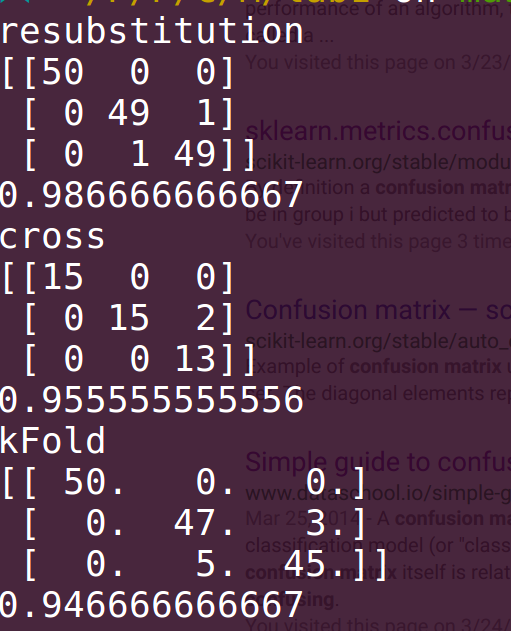
\includegraphics[width=6cm]{result.png}
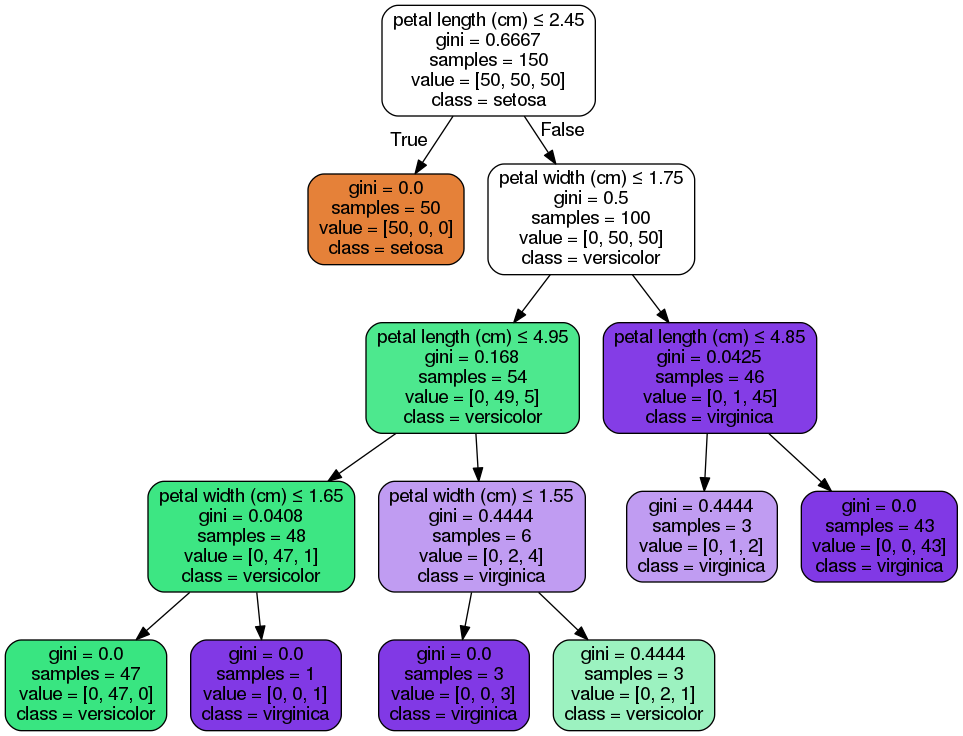
\includegraphics[width=10cm]{iris.png}
\section{Environment}
Ubuntu 16.04\\
python3.5
\section{Language and Library}
python 3.5\\
NumPy\\
SciPy\\
Scikit-learn\\
pydotplus\\
graphviz // apt(dnf) package
\section{How to used it}
  \begin{lstlisting}[language=bash]
    $ python3 iris.py
  \end{lstlisting}
\section{Code}
  decition tree 是用 scikit 提供的 decition tree 建的,其中僅對 feature 小於 5 個時停止往下長做調整,避免產生 overfitting 的結果

  在 resubstitution 時候直接將 data 丟入 decision tree 中做 trainning,然後又直接拿 data 去做 prediction,會得到一個 overfitting 的結果

  再做 cross validition 時,對 data 做 3:7 的分開,3\% 做 test data,剩下 7\% 做 training,會得到一個 90~95\% 準確率的 decition tree

  最後做 KFold 時,將測資分 12 區,每次建一個 decition tree,計算 confusion matrix 並加總,最後在計算加總的 matrix 的準確率大概也是 90~95\%,其中要記得若中間的 confusion matrix 並非 $3\times3$ 的 matrix 的話,需要補滿 0 以成為 $3\times3$ 的 matrix
\end{CJK}
\end{document}
